%=====================================================================
%==========================PAQUETES y DEFICION DEL ARCHIVO============
\documentclass[12pt]{article}
\usepackage[spanish,mexico]{babel}
	\selectlanguage{spanish}
\usepackage{graphicx}
\usepackage{amsmath}
\usepackage{wrapfig}
\usepackage{float}
\usepackage[utf8]{inputenc}
\usepackage[utf8]{inputenc}
\usepackage{color}
\usepackage{graphicx}
\graphicspath{{images/}}

\setlength{\parskip}{\medskipamount}
\setlength{\parindent}{0pt}
\definecolor{labelcolor}{RGB}{100,0,0}


\usepackage{vmargin}
\setmarginsrb{3 cm}{1.0 cm}{3 cm}{1.0 cm}{1 cm}{1.5 cm}{1 cm}{1.5 cm}
\usepackage{listings}
%=====================================================================
%=======================DATOS AUTOR===================================
%=====================================================================
\title{Actividad 8: Iniciandose en Computo Simbolico con Maxima}
\author{Martin Alejandro Paredes Sosa}
\date{Abril, 2016}
%=====================================================================
%=====================================================================
\begin{document}
\maketitle

\section{Introducción}
\section{Geometria en tres dimensiones}
Esta sección consta en enseñarnos herramientas para geometria tridimensional.
\subsection{Vectores y Algebra lineal}
Se aprendió a declarar vectores así como, algunas de las operaciones entre vectores como es el producto punto y el producto cruz.

\noindent
%====================================================
\noindent

\begin{minipage}[t]{8ex}{\color{red}\bf
\begin{verbatim}
(%i1) 
\end{verbatim}}
\end{minipage}
\begin{minipage}[t]{\textwidth}{\color{blue}
\begin{verbatim}
a: [6,2,5];
b: [8,-3,0];
a.b;
load(vect);
express(a~b);
c: [-5,2,9];
express(a.(b~c));
\end{verbatim}}
\end{minipage}

\begin{math}\displaystyle
\parbox{8ex}{\color{labelcolor}(\%o1) }
[6,2,5]
\end{math}

\begin{math}\displaystyle
\parbox{8ex}{\color{labelcolor}(\%o2) }
[8,−3,0]
\end{math}

\begin{math}\displaystyle
\parbox{8ex}{\color{labelcolor}(\%o3) }
42
\end{math}

\begin{math}\displaystyle
\parbox{8ex}{\color{labelcolor}(\%o4) }
/usr/share/maxima/5.34.1/share/vector/vect.mac
\end{math}

\begin{math}\displaystyle
\parbox{8ex}{\color{labelcolor}(\%o5) }
[15,40,−34]
\end{math}

\begin{math}\displaystyle
\parbox{8ex}{\color{labelcolor}(\%o6) }
[−5,2,9]
\end{math}

\begin{math}\displaystyle
\parbox{8ex}{\color{labelcolor}(\%o7) }
−301
\end{math}


\subsection{Lineas, Planos y Superficies Cuadraticas}
Se definieron ecuaciones de planos y superficies, con el objetivo de poder visualizarlos.
\begin{minipage}[t]{8ex}{\color{red}\bf
\begin{verbatim}
(%i1) 
\end{verbatim}}
\end{minipage}
\begin{minipage}[t]{\textwidth}{\color{blue}
\begin{verbatim}
load(draw);
ellips1: x^2/3+0.5*x*y+z   = 0;
draw3d(enhanced3d = true,
       palette = [cyan,blue,cyan],
       implicit(ellips1, x,-100,100, y,-100,100, z,-100,100));
\end{verbatim}}
\end{minipage}

\begin{math}\displaystyle
\parbox{8ex}{\color{labelcolor}(\%o1) }
/usr/share/maxima/5.34.1/share/draw/draw.lisp
\end{math}

\begin{math}\displaystyle
\parbox{8ex}{\color{labelcolor}(\%o2) }
z+0.5\,x\,y+\frac{{x}^{2}}{3}=0
\end{math}

\begin{math}\displaystyle
\parbox{8ex}{\color{labelcolor}(\%o3) }
[\mathrm{gr3d}\left( implicit\right) ]
\end{math}
\begin{figure}[H]
\centering
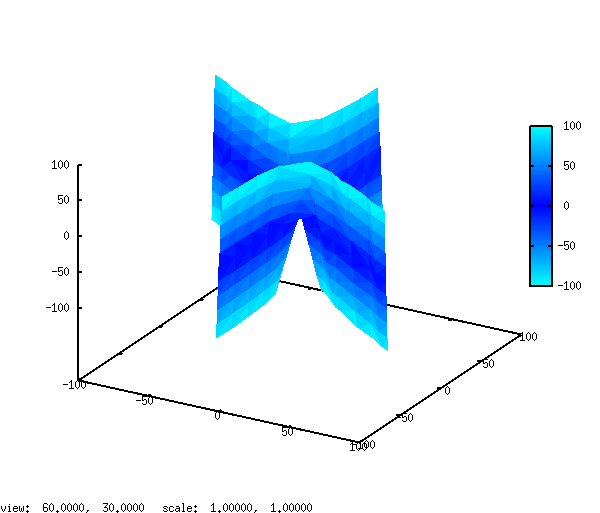
\includegraphics[scale=0.75]{1.png}
\caption{Grafica de la superficie $z+0.5\,x\,y+\frac{{x}^{2}}{3}=0$}
\end{figure}
\subsection{Funciones Vectoriales}
\subsection{Longitud de Arco y Curvatura}


\end{document}